%; whizzy chapter -dvi
% -initex iniptex -latex platex -format platex -bibtex jbibtex -fmt fmt
% 以上 whizzytex を使用する場合の設定。

%     Tokyo Debian Meeting resources
%     Copyright (C) 2012 Junichi Uekawa
%     Copyright (C) 2011 Nobuhiro Iwamatsu

%     This program is free software; you can redistribute it and/or modify
%     it under the terms of the GNU General Public License as published by
%     the Free Software Foundation; either version 2 of the License, or
%     (at your option) any later version.

%     This program is distributed in the hope that it will be useful,
%     but WITHOUT ANY WARRANTY; without even the implied warranty of
%     MERCHANTABILITY or FITNESS FOR A PARTICULAR PURPOSE.  See the
%     GNU General Public License for more details.

%     You should have received a copy of the GNU General Public License
%     along with this program; if not, write to the Free Software
%     Foundation, Inc., 51 Franklin St, Fifth Floor, Boston, MA  02110-1301 USA

%  preview (shell-command (concat "evince " (replace-regexp-in-string "tex$" "pdf"(buffer-file-name)) "&"))
% 画像ファイルを処理するためにはebbを利用してboundingboxを作成。
%(shell-command "cd image201307; ebb *.jpg")

%%ここからヘッダ開始。

\documentclass[mingoth,a4paper]{jsarticle}
\usepackage{monthlyreport}

% 日付を定義する、毎月変わります。
\newcommand{\debmtgyear}{2013}
\newcommand{\debmtgmonth}{8}
\newcommand{\debmtgdate}{17}
% started from zero:
% (let ((year 2013) (month 7)) (+ (* (- year 2005) 12) month -1))
\newcommand{\debmtgnumber}{103}

\begin{document}

\begin{titlepage}
\thispagestyle{empty}
% タイトルページ:編集必要な部分は最初のマクロに飛ばすこと

\vspace*{-2cm}
第\debmtgnumber{}回 東京エリア Debian 勉強会資料\\
\hspace*{-2cm}

\includegraphics{image2012-natsu/dotdeb.pdf}\\
\hfill{}\debmtgyear{}年\debmtgmonth{}月\debmtgdate{}日

% ここはアップデートすること
% 全角文字にしないとフォントのサイズが合わないので注意
\rotatebox{10}{\fontsize{32}{32} {\gt 特集1: OpenVPNを使ってみた }}

\rotatebox{10}{\fontsize{32}{32} {\gt 特集2: 
デビアン勉強会資料のePUB化}}

\vspace*{-2cm}
\hfill{}
\includegraphics[height=6cm]{image200502/openlogo-nd.eps}
\end{titlepage}

\newpage

\begin{minipage}[b]{0.2\hsize}
 \definecolor{titleback}{gray}{0.9}
 \colorbox{titleback}{\rotatebox{90}{\fontsize{80}{80} {\gt デビアン勉強会} }}
\end{minipage}
\begin{minipage}[b]{0.8\hsize}
\hrule
\vspace{2mm}
\hrule
\begin{multicols}{2}
\tableofcontents
\end{multicols}
\vspace{2mm}
\hrule
\end{minipage}

\dancersection{事前課題}{上川 純一}

今回の事前課題は以下です:
\begin{enumerate}
 \item 自分では vpn をどう利用していますか?
\end{enumerate}
この課題に対して提出いただいた内容は以下です。
\begin{multicols}{2}
{\small
 
\begin{prework}{ Yoshida Shin }

VPN を構築した事は有りません。
また、プライベートでも使用した事は有りません。

VPN は仕事で以下の 2個の使い方をしています。
\begin{enumerate}
 \item  データセンターのサーバーにログインする
 \item  緊急対応のため、自宅から職場につなぐ
\end{enumerate}

でも、緊急対応は行わないで済むようにするべきだし、
(緊急対応が無いと仮定すれば、)多くの場合はデータセンターへの接続も
職場からの IP 制限だけで十分だと考えています。

VPN は万一の為に用意するものであり、
あまり積極的に使いたいと思わないです。
\end{prework}

\begin{prework}{ 吉野(yy\_{}y\_{}ja\_{}jp) }

個人的には使ってません.
\end{prework}

\begin{prework}{ sakai }

今のところVPNは利用していない。
そのうち、外出した時用にVPNで自宅とつなごうかなー、ということを考える程度。
\end{prework}

\begin{prework}{ 野島 貴英 }

以前、苦肉の策で2つの拠点間をインターネット経由でopenvpn使って一時的にLANを組み、複数のWEBサイトのWEB-DB間のアクセスを遠方のDBに常時流し込みつづけてそのまま半月ぐらいサービス維持した事があります。使った結果ですが、予想外にも、簡単/大変タフ/非常に安定したVPN経路が組めた記憶があります。ただ、ちゃんとしたデータ取ってないので、感想以上の事がいえない状況ではあります。
\end{prework}

\begin{prework}{ dictoss(杉本 典充) }

最近自宅サーバにopenvpnを入れて、出先でテザリングをしながらサーバにアクセスしている。
それまではsshとポートフォワードでがんばっていたが、サーバの台数が増えるとポートフォワードの数が増えるので設定が疲れました。
VPSから自宅サーバにVPNセッションを張ろうかと思っているが自宅サーバはDynamicDNSを利用しているので切れずにつながっていられるか不明。

会社だと拠点間をつなぐためにL2TP/IPsecでVPNを張る場合や、グロバールIPを持たない(=NAT配下)に設置されるが管理上サーバからsshする必要があるPCにはクライアントからVPNを張らせることでsshできるようにする、といった使い方をしている。
\end{prework}

\begin{prework}{ まえだこうへい }

会社環境に繋ぐのに、OpenVPNと、Cisco Anycoonect を使ってますが、後者の環境では、Anyconnectクライアントではなく、OpenConnectを使ってます。RSA OneTimePasswordのモジュールを併用して二要素認証にしていますが、これにも対応してます。

個人環境ではSSHのProxy機能を使っているので、接続先ノード数増えても特に困らずVPNって面倒だよなぁとふと思い出しながら仕事してます。
\end{prework}

}
\end{multicols}

\dancersection{Debian Trivia Quiz}{上川純一}

ところで、みなさん Debian 関連の話題においついていますか?Debian関連の話
題はメーリングリストをよんでいると追跡できます。ただよんでいるだけではは
りあいがないので、理解度のテストをします。特に一人だけでは意味がわからな
いところもあるかも知れません。みんなで一緒に読んでみましょう。

今回の出題範囲は\url{debian-devel-announce@lists.debian.org} や \url{debian-devel@lists.debian.org}に投稿された
内容とDebian Project Newsからです。

\begin{multicols}{2}
 %; whizzy-master ../debianmeetingresume201308.tex
% 以上の設定をしているため、このファイルで M-x whizzytex すると、whizzytexが利用できます。
%

\santaku
{Sylvestre Ledru が JDK についてアナウンスしたのは}
{OpenJDK7にきりかえ}
{JDK6の削除}
{JDK8への移行}
{A}
{java-commonをOpenJDK 7 に切り替えるそうですよ、しかし一部のアーキテクチャ
はOpenJDK 6のまま。}

\santaku
{OpenJDK7でサポートされていないアーキテクチャはどれか}
{mipsel}
{amd64}
{i386}
{A}
{s390, mips, mipsel, kfreebsd, sparcがサポートされていないようです。}

\santaku
{Summer Of Code のコーディネーションメンバーでないのは誰か}
{David Bremner}
{Nicolas Dandrimont}
{Nobuhiro Iwamatsu}
{C}
{例年Summer of code スポンサーで開発する内容を調整するボランティアがいま
す。}

\santaku
{Brian GuptaがDebianのトレードマークとしてUSPTOに追加登録しようと提案したのは何か}
{ロゴ}
{Debianの文字列}
{DD}
{A}
{`Debian' は登録されていたがロゴは登録されていなかったので登録することに
したようです。}


\end{multicols}

\dancersection{最近のDebian関連のミーティング報告}{上川純一}
\subsection{東京エリアDebian勉強会102回目報告}

東京エリアDebian勉強会102回めは杉並区荻窪で開催されました。

岩松さんが Linux Kernel の armmp フレーバーについて紹介しました。
デバイスツリー情報を利用することで複数のボードをサポートする仕組みのよう
です。

野島さんがdh\_stripについて紹介しました。デバッグ情報について深いお話で
した。

上川がraspberry piを使ってみたのでその紹介をしました。

% (query-replace-regexp "<.*?>" "")
% (query-replace-regexp "^[	 ]\+" "")

%-------------------------------------------------------------------------------
\dancersection{OpenVPNを使ってみた}{上川純一}
%-------------------------------------------------------------------------------
\index{openvpn}

\subsection{はじめに}

VPN(仮想プライベートネットワーク)とはインターネット上にある(WAN)に閉域ネットワー
ク(LAN)を仮想的に構築する方法です。

OpenVPNは認証と接続方式の部分でTLS\cite{rfc5246} \footnote{規格がTLSにな
るまえはSSLという規格でした}を活用しています。TLSはHTTPSなど
で利用されている仕組みで、公開鍵認証をつかって最初の鍵交換をおこな
い、そこで交換した対象鍵をつかって実際の通信をすることで効率良く暗号通信ができる
ようになっています。

\subsection{今回実現したいこと}

今回想定する例としてとある個人の開発環境ネットワーク構成図を見てみましょ
う(\fgref{fig:network})。

自宅にはごく一般的なプロバイダ契約でネットワークをひいていて、ラッ
プトップと携帯電話はどういうネットワークを経由してどういうIPアドレスでつ
ながるのかよくわからないという構成です。

携帯電話とラップトップから自宅にあるサーバ Raspberry Pi にアクセスできる
ようにしたい、そう思った時にプライベートIPで接続しているプロバイダー接続がネッ
クになります。

開発や実験などに便利な環境を実現したい、それはRaspberry pi とラップトップ
と携帯電話が同じLANにいるような環境です。

\begin{figure}[H]
\begin{center}
  \includegraphics[width=0.8\hsize]{image201308/network.eps}
 \caption{とある個人の開発環境ネットワーク構成図}
 \label{fig:network}
\end{center}
\end{figure}

\subsection{OpenSSL, CA の仕組み}

OpenVPN で利用できる認証のしくみは複数あり、一番簡単な方法は共有鍵方式だ
と思われます\footnote{認証なし暗号化なしという方法もあってそっちのほうが
簡単ですがopenvpnの接続性テスト以外ではあまりつかわないと思います}。ここ
では自分の直接の管理下にあるマシンを複数台管理する場合に便利そうな方式、
自前でCAを立ててPKI(x509)で構築する方法について紹介します。

今回紹介する方式を実現する副作用として、openvpnに脆弱性があったり、認証情
報がもれると外部のユーザが仮想のプライベートネットワークに接続できるよう
になります。また、ネットワークにはユーザ認証がないので、VPN接続しているホ
ストにログインできればプライベートネットワークにアクセスできるようになり
ます。

\subsection{インストール}

Debianでは openvpnパッケージとして提供されています。また、CA関連はopensslに依存
しているのでopensslパッケージもインストールしましょう。

\begin{commandline}
 # apt-get install openvpn openssl
\end{commandline}

\url{/etc/openvpn/*.conf} に設定ファイルを配置します。 Debianでのopenvpn
の設定は、/etc/openvpnディレクトリにあるconfという拡張子に
なっているファイルを設定ファイルとして認識して起動時に利用するようです。
デフォルトの状態では、最初は何も設定ファイルがないので何も起動していませ
ん。

クライアント側もopenvpnパッケージをインストールします。

\subsection{OpenVPNの接続性試験}

まず、サーバとクライアント間で接続できるかどうかを確認する方法について紹
介します。サーバとクライアントでopenvpn を起動して相互に接続し、openvpnが
接続できる状態であることを確認します。pingとかうってみるのがよいでしょう。

openVPN は UDP もしくは TCP 接続を利用することができます。どちらかはつな
がるでしょう。

\begin{commandline}
 server$ sudo openvpn --dev tun1 --ifconfig 10.1.1.1 10.1.1.2 
 client$ sudo openvpn --dev tun1 --remote サーバホスト名 --ifconfig 10.1.1.2 10.1.1.1 

 client$ ifconfig
 tun1      Link encap:UNSPEC  HWaddr 00-00-00-00-00-00-00-00-00-00-00-00-00-00-00-00  
          inet addr:10.1.1.2  P-t-P:10.1.1.1  Mask:255.255.255.255
          UP POINTOPOINT RUNNING NOARP MULTICAST  MTU:1500  Metric:1
          RX packets:2 errors:0 dropped:0 overruns:0 frame:0
          TX packets:2 errors:0 dropped:0 overruns:0 carrier:0
          collisions:0 txqueuelen:100 
          RX bytes:168 (168.0 B)  TX bytes:168 (168.0 B)
 client$ ping 10.1.1.1

\end{commandline}

\subsection{CAの作成}

まず最初に認証局を作成します。
とりあえずは easy-rsa を使うとよいでしょう。wheezy のopenvpnパッケージでは
\url{/usr/share/doc/openvpn/examples/easy-rsa/2.0/}にファイルがおいてありそれ
をコピーしてつかえということのようです。

\begin{commandline}
 # cd /etc/openvpn
 # sudo cp -R /usr/share/doc/openvpn/examples/easy-rsa/2.0/ easy-rsa/
 # cd easy-rsa/
 # vi vars

export KEY_COUNTRY="JP"
export KEY_PROVINCE="TOKYO"
export KEY_CITY="Suginami-ku"
export KEY_ORG="uekawa"
export KEY_EMAIL="dancerj@gmail.com"
#export KEY_CN=changeme
#export KEY_NAME=changeme
#export KEY_OU=changeme
#export PKCS11_MODULE_PATH=changeme
#export PKCS11_PIN=1234

 # . ./vars
 # ./clean-all
 # ./build-ca
 
\end{commandline}

いろいろと質問されますが、あまり重要な質問はない気がします。
``Common Name''が名前で、ここで聞かれている名前はCAの名前です。が、この
名前が重要な場面はあまりない気がします。

注意事項としては何も設定しないと全員ファイルが読めるようになっているので
すが、認証情報関連のファイルは秘密であることが重要なので、rootのみが読め
るようにしましょう。

\subsection{各種証明書の作成}

サーバはクライアントが信頼できるCAに署名された証明書を使っていることを確
認することになります。クライアントはサーバの証明書が信頼できるCAにに署名
されていることを確認することになります。

正式な手順はクライアント・サーバ各ノードで Certificate Signing Request
(CSR) を作ってCA側で署名してCRTファイルを返してあげるということになります。
今回は略式でサーバをCAとして運用し発行機関としても併用します。
OpenVPNサーバが乗っ取られたらCAとしても乗っ取られるのですがOpenVPNサーバ
が乗っ取られた時点で全ノードの再設定が必要になると思うので、新しく自己署
名CAを作りなおしてしまうという方針でいきます。

まずサーバの証明書を作成します。今回sakuraという名前のサーバの証明書を作っ
てみましょう。

\begin{commandline}
 # ./build-key-server sakura
\end{commandline}

CN(common name) のところにはホスト名をいれる慣習になっているようで、
その値は後々ログなどで表示されます。
A challenge password と an optional company name はCSRに追加ではいる情報
みたいですが、CSRを読むことはないのでこの場合は何も入力しなくてもよいよ
うです。
証明書を作成して証明書の署名と登録を連続しておこなうのでちょっとわかりに
くいです。

クライアントの証明書を作成します。
\begin{commandline}
 # ./build-key client1
 # ./build-key nexus4
\end{commandline}

\subsection{HMAC鍵の作成}

TLSをのハンドシェークはCPU負荷の高い処理なのでDoSされる可能性もあります。
そこで、HMAC鍵を使ってその前段でフィルタリングをかけることができるようで
す。ついでにつくってしまいましょう。

\begin{commandline}
 # openvpn --genkey --secret ta.key
\end{commandline}

\subsection{OpenVPNのサーバ設定}

TLS接続用にサーバ側で必要となる Diffie Hellman パラメータ(なにそれ?)を
生成します。

\begin{commandline}
 # ./build-dh  
\end{commandline}

\url{/etc/openvpn/server.conf}に設定ファイルを作成します。

\begin{commandline}
port 1194
proto udp
dev tun

user nobody
group nogroup

tls-auth      /etc/openvpn/easy-rsa/keys/ta.key 0 # server is 0.
ca      /etc/openvpn/easy-rsa/keys/ca.crt
cert    /etc/openvpn/easy-rsa/keys/sakura.crt
key     /etc/openvpn/easy-rsa/keys/sakura.key  # keep secret
dh      /etc/openvpn/easy-rsa/keys/dh1024.pem

server 10.55.2.0 255.255.255.0  # internal tun0 connection IP
ifconfig-pool-persist ipp.txt

keepalive 10 120

comp-lzo         # Compression - must be turned on at both end
persist-key
persist-tun

status log/openvpn-status.log

verb 3  # verbose mode
client-to-client
 
\end{commandline}

この設定ファイルはlog/ディレクトリにステータスログを出力する設定なので、
ディレクトリ \url{/etc/openvpn/log/} をつくっておきます。

/etc/openvpn/ipp.txt にIPアドレスの割り当て設定が記録されます。
デフォルトでは60秒に一回更新されるようになっています。

keepalive 10 120 の設定では、サーバとクライアントはお互いに10秒に一回
ping で生死監視をして、2分間接続がなかったら再起動します。

\url{ /etc/openvpn/*.conf} にファイルがあると起動時にサーバを起動してく
れるようになるのでこれで設定は完了です。

\subsubsection{トポロジー}

デフォルトのTUNデバイスのトポロジーは net30 です。これはクライアント毎に
サブネットマスク /30 の ipv4 アドレス(4個づつ)を割り当てることになります。
ブリッジモードでTAPを使う、もしくはp2p・subnetトポロジを使うとクライアン
トあたり一つのIPアドレスになるみたいですが、どうせクラスAのプライベート
アドレスを大量に使えるので特に必要もないので検証してません。

\subsubsection{tun or tap}

仮想ネットワークデバイスはTUNとTAPの二択あります。TAPはイーサネット
レベル(L2)の仮想デバイスで、TUNはIPレベル(L3)の仮想デバイスです。今回
はiOSと
AndroidのopenvpnクライアントがTUNしかサポートしていないのでTUNを使うこと
になります。

\begin{tabular}{|c|c|c|c|}
\hline
 & ネットワークレイヤー & 機能 & つかえるOS\\
\hline
tap & L2 & ブリッジ(ブロードキャストパケットが到達する) & linux \\
tun & L3 & ルータ & linux, iOS, Androidなど \\
\hline
\hline
\end{tabular}


\subsection{OpenVPNのクライアント設定}

CAからいくつかのファイルをコピーしてくる必要があります。Debianの場合はサー
バと大体ディレクトリ構成をあわせておけばよいでしょう。rootでしか読み込め
ないように権限を設定しておくのをお忘れなく。

ca.crt, client.crt, client.key, ta.key が必要になります。

Android の OpenVPN アプリケーションの場合\cite{openvpnconnectandroid}は、
\url{/sdcard} 以下に適当な名前でディレクトリを作成してそこに必要なファイ
ルを配置します。設定ファイルは拡張子をconfではなくovpnにしておかないと認
識してくれないようです。一回 OpenVPN アプリケーションでImportしたらその
SDカード上のディレクトリの中身は必要なくなるので消しましょう。

\begin{commandline}
client
dev tun
port 1194
proto udp

remote xyz.sakura.ne.jp 1194             # vpn server ip : port
nobind

tls-auth      ta.key 1 # client is 1.
ca ca.crt
cert android-nexus4.crt
key android-nexus4.key

remote-cert-tls server
comp-lzo
persist-key
persist-tun

verb 3

\end{commandline}

remote-cert-tls server で証明書がサーバー鍵であることを確認しま
す。./build-key-server で作られた証明書は ``key usage'' に サーバ証明書で
あることが記述されています。これを指定しないと有効なCAをに署名された証明
書であればどれでもつなぎに行きます。たとえば流出したクライアントの証明書
でサーバを偽装することが可能になります。

起動方法は、 \url{/etc/network/interfaces} に記述することもできますが
\cite{openvpnreadmedebian}デフォルトの状態でネットワークの設定が変更になっ
たら勝手に OpenVPN 接続を試行してくれる設定になっているようです。
\footnote{多分\url{/etc/network/if-up.d/openvpn}の設定による}

\subsubsection{Android UI}

Androidデバイスに必要なファイルをコピーします。
\begin{commandline}
$ ls -1 
android-nexus4.crt
android-nexus4.csr
android-nexus4.key
ca.crt
client.ovpn
ta.key
$ adb push . /sdcard/secure
push: ./ca.crt -> /sdcard/secure/ca.crt
push: ./android-nexus4.key -> /sdcard/secure/android-nexus4.key
push: ./ta.key -> /sdcard/secure/ta.key
push: ./android-nexus4.crt -> /sdcard/secure/android-nexus4.crt
push: ./client.ovpn -> /sdcard/secure/client.ovpn
push: ./android-nexus4.csr -> /sdcard/secure/android-nexus4.csr
\end{commandline}

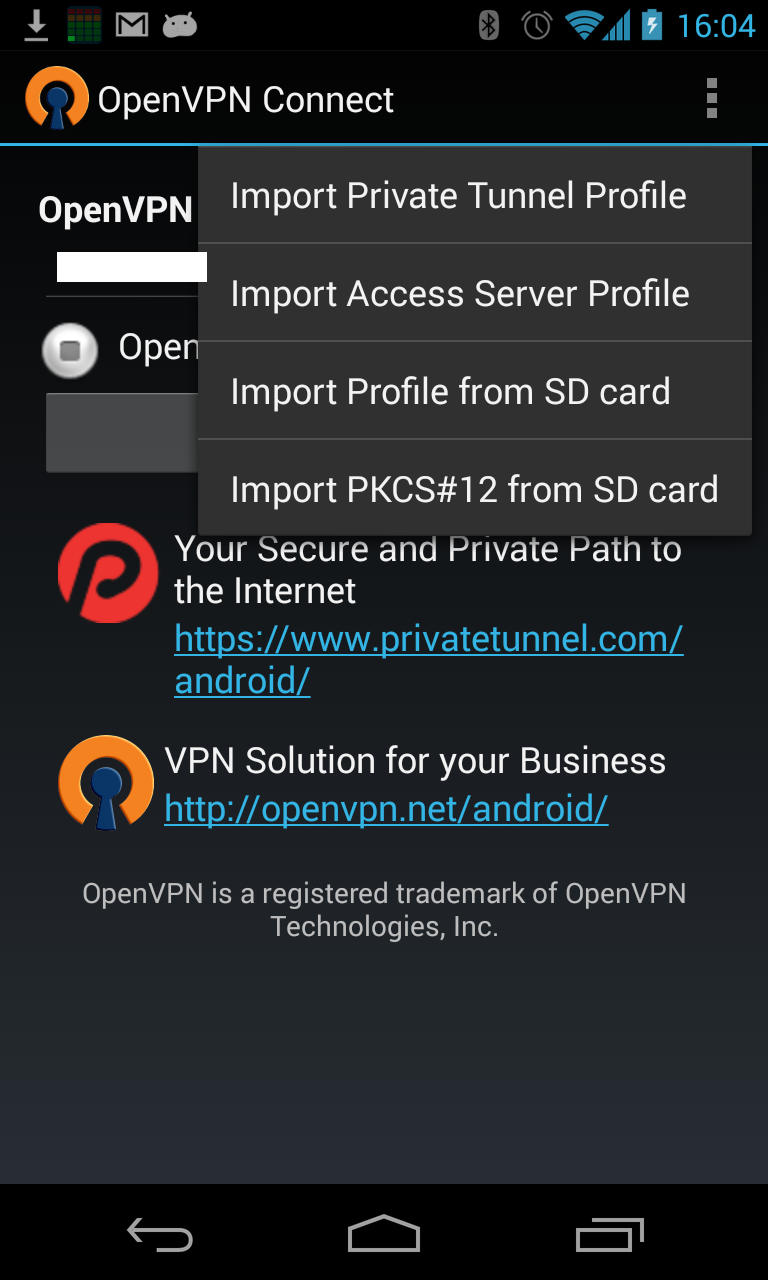
\includegraphics[width=0.3\hsize,bb=0 0 768 1280]{image201308/Screenshot_2013-08-17-16-04-31.png}
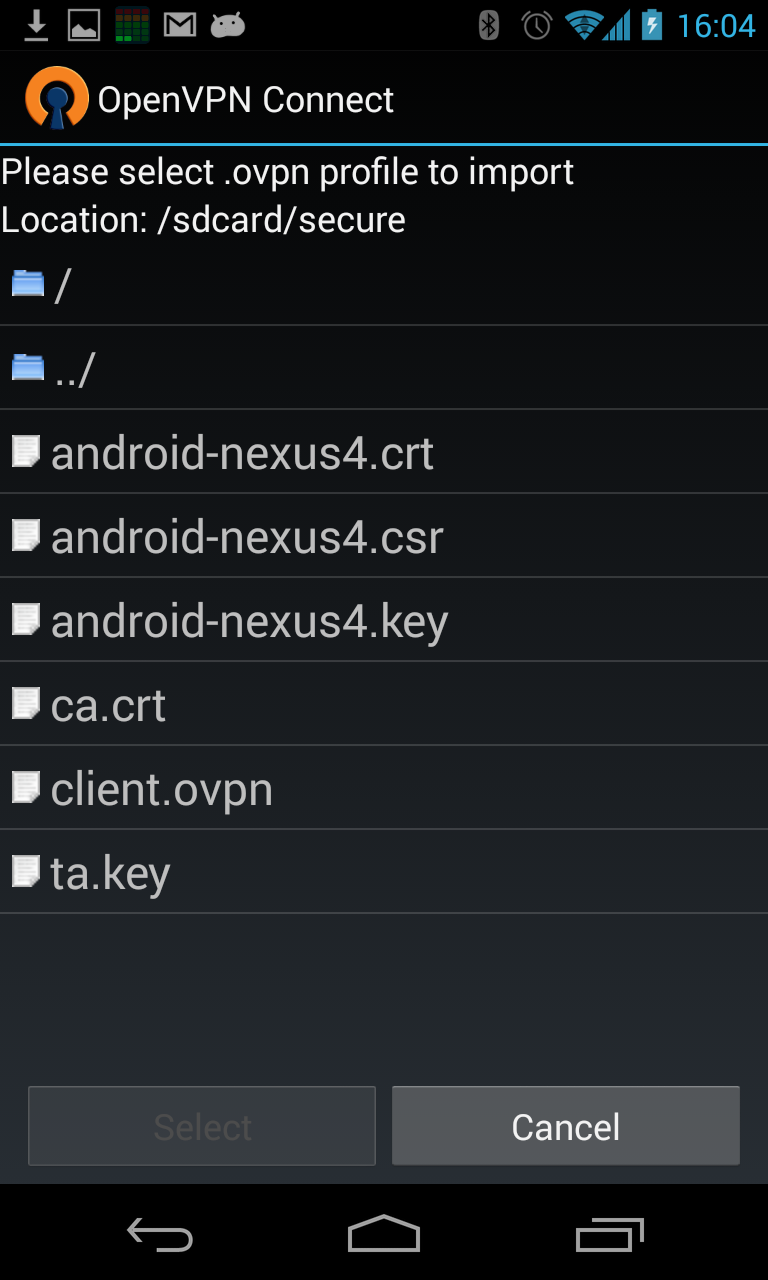
\includegraphics[width=0.3\hsize,bb=0 0 768 1280]{image201308/Screenshot_2013-08-17-16-04-43.png}
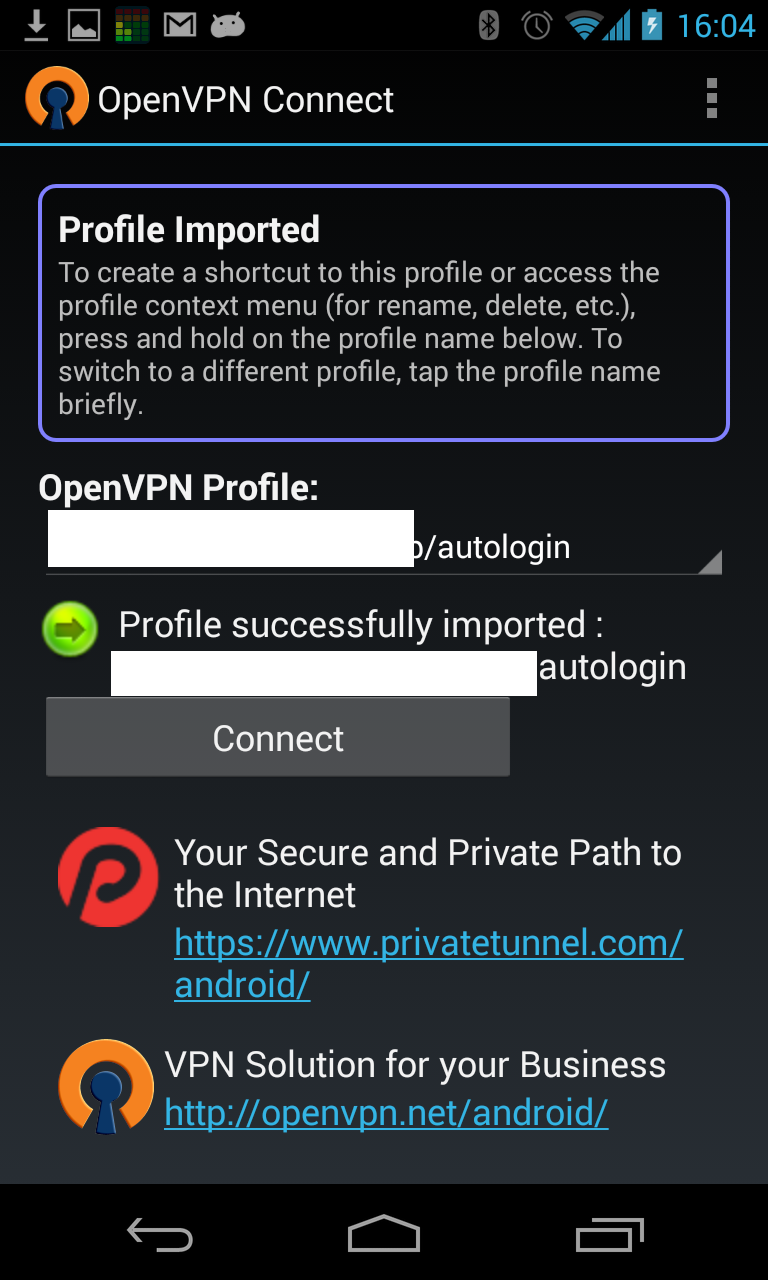
\includegraphics[width=0.3\hsize,bb=0 0 768 1280]{image201308/Screenshot_2013-08-17-16-04-54.png}
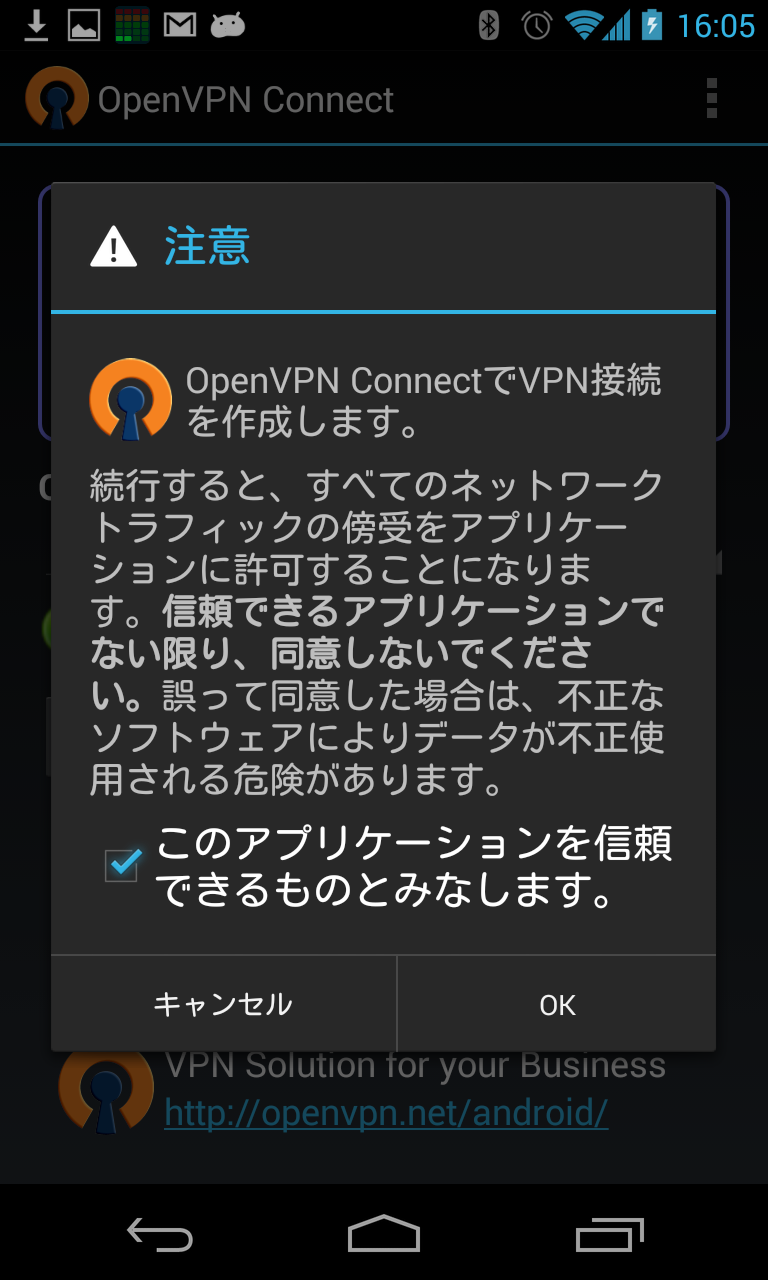
\includegraphics[width=0.3\hsize,bb=0 0 768 1280]{image201308/Screenshot_2013-08-17-16-05-07.png}

インポートしたらsdcardからファイルを削除します。

\subsection{応用}

特に今回必要でなかったので設定しなかったのですが違う設定も可能なのでそれ
も紹介します。

ルーティングなどは openvpn サーバ側で設定すればクライアントに設定を配布
(push)してくれるようです。

\subsubsection{ローカルネットワークへのゲートウェイを設定したい}

redirect-private オプションでVPN経由でのルーティングを設定します。
たとえば、VPN経由のゲートウェイ(たとえば 10.0.0.1) 経由で 自宅のネット
ワーク(例えば 192.168.1.0/24) にアクセスできるようにしたいときに使えま
す。

\url{/usr/share/doc/openvpn/examples/sample-config-files/firewall.sh}に
iptablesの設定例が掲載されています。

\subsubsection{暗号化経路のためにすべてのパケットをVPN経由にしたい}

redirect-gateway オプションで指定できます。

公共の WiFi スポット経由での通信などが安心できない人向けのオプションです。
しかしDHCPの再リースやDNSの名前解決などもVPN経由になってしまうと困る場合
もあるので bypass-dhcp, bypass-dns オプションなどがあるようです。

\subsection{おわりに}

openvpn 2.3 でgitリポジトリの再編を行ったようで、
easy-rsaとかが分離されたっぽいです。

マニュアルを読んでいるとWindows 版の専用オプションとかが複雑にからみあっ
ていて実際どれをつかえばよいのか読み解きにくいです。最低限動かすまではそ
こまで難しくないのですがルーティングとかデフォルトゲートウェイを変更し
ようかと考え始めると考えることがいくつかあるようです。
しかし一般論で考えても、ネットワーク3つ以上を接続する場合のファイアウォー
ルとかルーターの設定はそれなりに複雑ですから、それを考えると妥当なのかも
しれませんね。

\subsubsection{ssh の各機能との比較}

開発者・運用者愛用のツールsshとどう違うのかとおもってみてみたのですが、
sshにも VPN 機能もあるので比較しにくいですね。ただ、通常の運用ではroot同
士でsshすることはあまりないかと思いますが、VPNを利用するにはrootでssh で
きる必要があるようです。

openvpnのメリットとしては openvpn には接続が切れた時を検出して再接続する
仕組みがあること、TCPだけでなくUDPも使えること、root 権限でsshログインを
許可しないでよいことなどがあげられると思います。

\begin{table}[H]
 \caption{ssh の機能の対応}
 \begin{tabular}{|c|c|c|}
 \hline
 \hline
 & sshオプション & 機能 \\
 \hline
 ポートフォワーディング &  -L, -R & 特定のローカルのTCPポート番号をリモートのポート番
	 号とマッピングする \\
 \hline
 プロキシ & -D & SOCKSに対応しているアプリケーションのプロキシを提供 \\
 \hline
 VPN & -w & IPレベルで相互に見えるよう仮想的にネットワークを構築する \\
 \hline
 \hline
 \end{tabular}
\end{table}


\begin{thebibliography}{0}
 \bibitem{openvpndebianwiki} \url{http://wiki.debian.org/OpenVPN}
 \bibitem{openvpnmanpage} openvpn(8) manpage
 \bibitem{openvpnreadmedebian} OpenVPN README.Debian \url{/usr/share/doc/openvpn/README.Debian.gz}
 \bibitem{openvpnnetcommunity} OpenVPN Community Software
	 \url{http://openvpn.net/index.php/open-source.html}
 \bibitem{rfc5246}               
	 The Transport Layer Security (TLS) Protocol
	 Version 1.2
	 \url{https://tools.ietf.org/html/rfc5246}
\bibitem{openvpnconnectandroid} OpenVPN Connect Android app
	\url{https://play.google.com/store/apps/details?id=net.openvpn.openvpn}
\end{thebibliography}

%-------------------------------------------------------------------------------
\dancersection{Debian勉強会の資料のePUB化を試みた}{まえだこうへい}
%-------------------------------------------------------------------------------
\index{epub}
\index{latex}
\index{pdf}

\subsection{ePUB化の動機}

最近はかなりスマートフォンやタブレットが普及し、それ以外のeBook readerも東京周辺の電車内でも見かけるようになりました。Debian勉強会の参加者もそれらのデバイスを持っている人も今までちらほら見かけています。Debian勉強会の事前配布資料や年2回の「あんどきゅめんてっどでびあん\footnote{現在名前は違いますが、これが一番通りは良いと思うのでこのまま表記します。}」をそれらのデバイスで読む機会も増えているのではないでしょうか。

ところで、Debian勉強会の資料はLaTeXをソースとしてPDFとして配布されています。PDFは印刷物と同じレイアウトになるので、本勉強会のように印刷した資料を頒布する上では最適です。しかし、画面で閲覧するのには向いていないと思いませんか。その一番の理由は多くのPDFリーダーは、画面に最適な大きさで自動的にリサイズされないためだと考えています。\footnote{ここでは印刷物に比べて読みにくい、という観点では論じません。}読みたい部分を拡大表示することはできますが、画面サイズに合わせた文字が巻き返しはされず、画面外にでた続きの文章は横方向にスクロールしなくてはなりません。これは面倒です。

そこでePUBです。O'Reilly, 達人出版会から出版されているEbookの多くはePUBが採用されているので、これらを既に購入、読んでいる人もいるでしょう。ページあたりの構成が画面サイズに最適化され、かつ、フォントサイズの変更でもページが自動的にリサイズされるので、これらのデバイスで読むのにはうってつけでしょう。

今回はDebian勉強会の資料を、LaTeXのソースコードには極力手を加えずに\footnote{PDFは今まで通り印刷物用に必要なので。}ePUB生成できないか検証しました。

\subsection{LaTeXからのePUB生成の方法}

\LaTeX から ePUBを生成するにはいくかの方法があります。取りうる手段としては4パターンです。

\begin{itemize}
  \item[1)] \LaTeX から直接 ePUBを生成する
  \item[2)] a. TeX もしくは b. DVIから, XMLもしくはHTMLを生成し、2)-2. ePUBに変換する
  \item[3)] PDFからePUBに変換する
\end{itemize}

\begin{figure}[H]
\begin{center}
  \includegraphics[width=0.7\hsize]{image201308/latex-epub.eps}
 \caption{LaTeXからePUBへの変換}
 \label{fig:convert-latex-to-epub}
\end{center}
\end{figure}

これらを行うためのツールについて検証しました。

\subsection{検証結果}

基本的にDebianパッケージになっているツールで検証を行いました。
対象は次の2つのファイルです。

\begin{enumerate}
  \item Debian勉強会の資料 (debianmeetingresume2013007.tex)
  \item latex2epubのサンプル \TeX ファイル (sample.tex)
\end{enumerate}

その結果は下記の通りです。

{\small
\begin{tabular}{|c|c|c|c|c|c}
\hline
パターン & ツール名 & 入力 & 出力 & \multicolumn{2}{|c|}{結果} \\ \cline{1-4}
 & & & & Debian勉強会の資料 & latex2pub のサンプル \\
\hline
1) & Pandoc & \LaTeX & ePUB & NG & OK \\
1) & latex2epub & \LaTeX & ePUB & NG & OK \\
2)-a & \LaTeX ML & \LaTeX & XML & NG & OK \\
2)-b & \TeX4ht & DVI & HTML & NG & NG \\
2)-b & htplatex(\TeX4ht) & \TeX & HTML & OK & NG \\
3) & Pandoc & HTML & ePUB & OK & N/A \\
4) & Calibre & PDF & ePUB & OK & OK \\
\hline
\end{tabular}
}


Debian勉強会の資料と、latex2epupのサンプル(以後、サンプルファイル)とで結果に大きな差がありますが、エラーメッセージを見る限りでは、その主な原因は使用しているdocumentclassの違いと、マクロの有無によるものではないかと考えられます。が、ここはあまり深堀できていません。

\subsection{変換できたケースでの課題}

Debian勉強会の資料で変換できたケースでの課題を挙げます。

\subsubsection{htplatex \& pandoc}

現状では次の問題がありますが、今回検証した中では一番まともに読める形で変換することができました。

\begin{itemize}
  \item tabularがtableに変換されず、表にならない
  \item 表紙の画像が追加されない
  \item あんどきゅめんてっどでびあん夏号、冬号をそれが含まれる月よりも先に変換すると、その中で使われている画像がhtmlディレクトリにコピーされず、ファイルが無いためpandoc実行時に失敗する
  \item \TeX4htでHTML変換時に自動生成される画像のファイル名が異なり、同じくpandoc実行時に失敗する月もある(2013年4月など)
  \item PDFを生成する場合(= makeを実行する場合)、htplatexが依存するパッケージ dvi2ps-fontdata-a2n をアンインストールする必要がある。これをアンインストールしないと、dvipdfmxでのDVIからPDF変換時に、"\texttt{** ERROR ** Virtual fonts nested too deeply}"というエラーが出て失敗する
\end{itemize}

なお、\TeX4ht は、実は上川さんが既に通った道でした。\footnote{\url{http://lists.debian.or.jp/debian-users/200708/msg00110.html}}
Debian勉強会の資料のリポジトリの中に、htplatexというシェルスクリプトがあります。
このスクリプトはDebian勉強会の資料の \LaTeX のファイルを \TeX4htを使ってHTML化するものです。

このスクリプトを使った手順は次のとおりです。

このスクリプトの2行目に使い方、3行目に依存パッケージのインストールについて記載されています。
まず、必要なパッケージをインストールします。

\begin{commandline}
$ apt-get install dvi2ps-fontdata-a2n dvi2dvi dvipng
\end{commandline}

次にスクリプトを実行します。

\begin{commandline}
$ ./htplatex debianmeetingresume200708.tex jp,2,sections+
\end{commandline}

すると、./html/ディレクトリ下に \LaTeX から変換されたHTMLが生成されます。
これをpandocを使ってePUBに変更します。

\begin{commandline}
$ cd html
$ pandoc -o debianmeetingresume200708.epub debianmeetingresume200708*.html
\end{commandline}

なお、このスクリプトは実行時に、"\texttt{-e}"オプションをつけることで、ePUBを生成することができるようにしました。

\begin{commandline}
$ ./htplatex -e debianmeetingresume200708.tex jp,2,sections+
\end{commandline}

変更内容は下記リンク先をご参照下さい。

\url{http://goo.gl/2KshN0}

\subsubsection{calibre}

calibreでは次の課題があります。

\begin{itemize}
  \item 目次のレイアウトが崩れる
  \item デフォルトでは行間が広すぎる
  \item 図が表示されない場合もある
  \item tabularが表として表示されない
\end{itemize}
変換時に、"ヒューリスティック処理を有効にする"にチェックを入れ、"外観"の"段落の間の間隔を削除する"にチェックを入れると、一部は多少改善されます。

\subsection{結論}
現時点では、 \LaTeX からのePUB生成は、不完全ながらも一応可能なようです。どれを選択するかはユーザ次第ではありますが、
いずれにしても更に使えるようにするには、各ツールでのパターンマッチングの機能を充実させる必要があるのではないかと思います。

しかし、iPad miniくらいの大きさのデバイスでは、Debian勉強会の資料のPDF版でもギリギリ拡大させなくても読めてしまいます。
ですので、PDFをそのまま読むのが一番読みやすい、という状況を解消できるようにしていくのが、我々の今後のアクションとなるに違いないでしょう。

\begin{thebibliography}{0}
 \bibitem{whatsthebesttextohtmlepubconverter} What’s the best \TeX-to-HTML or \TeX-to-ePUB converter?
   \url{http://boolesrings.org/krautzberger/2013/01/05/whats-the-best-tex-to-html-or-tex-to-epub-converter/}
 \bibitem{toolsforcovertinglatextoxml} Tools for Converting \LaTeX to XML
   \url{http://jblevins.org/log/xml-tools}
 \bibitem{pandoc} Pandoc \url{http://johnmacfarlane.net/pandoc/README.html}
 \bibitem{lxir} LXir \url{http://www.lxir-latex.org/}
 \bibitem{hermes} Hermes \url{http://hermes.roua.org/}
 \bibitem{texwiki} \TeX Wiki \url{http://oku.edu.mie-u.ac.jp/~okumura/texwiki/}
 \bibitem{tex4ht} \LaTeX をウエッブに載せよう
   \url{http://osksn2.hep.sci.osaka-u.ac.jp/~naga/miscellaneous/tex4ht/tex4ht-howto.html}
 \bibitem{latex2epub} \LaTeX2EPUB \url{http://kmuto.jp/d/index.cgi/computer/latex2epub.htm}
\end{thebibliography}

% \printindex

\cleartooddpage

\vspace*{15cm}
\hrule
\vspace{2mm}

\includegraphics[width=2cm]{image200502/openlogo-nd.eps}
\noindent \Large \bf Debian 勉強会資料\\
\noindent \normalfont \debmtgyear{}年\debmtgmonth{}月\debmtgdate{}日 \hspace{5mm}  初版第1刷発行\\
\noindent \normalfont 東京エリア Debian 勉強会 (編集・印刷・発行)\\
\hrule

\end{document}
